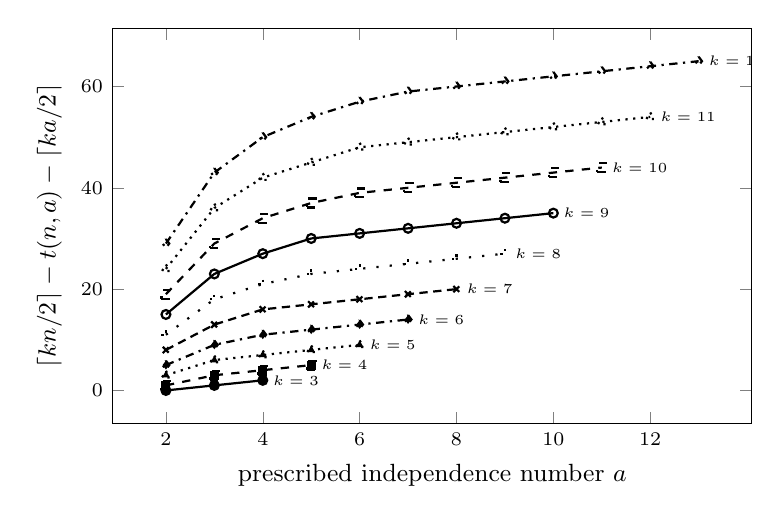
\begin{tikzpicture}
\begin{axis}[width=0.8\textwidth,height=6.6cm,xlabel={prescribed independence number $a$},ylabel={$\lceil kn/2\rceil-t(n,a)-\lceil ka/2\rceil$},tick label style={font=\scriptsize},label style={font=\small},xtick={2,4,6,8,10,12},cycle list={{solid,mark=*},{dashed,mark=square*},{dotted,mark=triangle*},{dashdotted,mark=diamond*},{densely dashed,mark=x},{loosely dotted,mark=+},{solid,mark=o},{dashed,mark=square},{dotted,mark=triangle},{dashdotted,mark=diamond}},every axis plot/.append style={line width=0.8pt}]
\addplot+[mark size=1.6pt] coordinates {(2,0) (3,1) (4,2)} node[pos=1,anchor=west,font=\tiny] {$k=3$};
\addplot+[mark size=1.6pt] coordinates {(2,1) (3,3) (4,4) (5,5)} node[pos=1,anchor=west,font=\tiny] {$k=4$};
\addplot+[mark size=1.6pt] coordinates {(2,3) (3,6) (4,7) (5,8) (6,9)} node[pos=1,anchor=west,font=\tiny] {$k=5$};
\addplot+[mark size=1.6pt] coordinates {(2,5) (3,9) (4,11) (5,12) (6,13) (7,14)} node[pos=1,anchor=west,font=\tiny] {$k=6$};
\addplot+[mark size=1.6pt] coordinates {(2,8) (3,13) (4,16) (5,17) (6,18) (7,19) (8,20)} node[pos=1,anchor=west,font=\tiny] {$k=7$};
\addplot+[mark size=1.6pt] coordinates {(2,11) (3,18) (4,21) (5,23) (6,24) (7,25) (8,26) (9,27)} node[pos=1,anchor=west,font=\tiny] {$k=8$};
\addplot+[mark size=1.6pt] coordinates {(2,15) (3,23) (4,27) (5,30) (6,31) (7,32) (8,33) (9,34) (10,35)} node[pos=1,anchor=west,font=\tiny] {$k=9$};
\addplot+[mark size=1.6pt] coordinates {(2,19) (3,29) (4,34) (5,37) (6,39) (7,40) (8,41) (9,42) (10,43) (11,44)} node[pos=1,anchor=west,font=\tiny] {$k=10$};
\addplot+[mark size=1.6pt] coordinates {(2,24) (3,36) (4,42) (5,45) (6,48) (7,49) (8,50) (9,51) (10,52) (11,53) (12,54)} node[pos=1,anchor=west,font=\tiny] {$k=11$};
\addplot+[mark size=1.6pt] coordinates {(2,29) (3,43) (4,50) (5,54) (6,57) (7,59) (8,60) (9,61) (10,62) (11,63) (12,64) (13,65)} node[pos=1,anchor=west,font=\tiny] {$k=12$};
\end{axis}
\end{tikzpicture}
